\section{Komplexe Folgen}

\subsection{Komplexe Folgen und ihr Verhalten im Unendlichen}

\begin{bsp}
    {Komplexe Folgen in Geogebra untersuchen}{}
    Im Unterricht werden die beiden Folgen $$z_1 = i, \quad z_{n+1} = z_n + 0.5$$ und $$z_1 = -1,\quad  z_{n+1} = z_n + 1.1^n \cdot \cis\left(\frac{\pi}{10}\right)$$ untersucht.

    Merke:
    \begin{itemize}
        \item  A2 ist ein relativer Zellverweis. Beim Kopieren einer solchen Zelle wird der Zellverweis angepasst.
        \item \$A\$2 ist ein absoluter Zellverweis. Beim Kopieren einer solchen Zelle bleibt der Zellverweis immer gleich.
    \end{itemize}
\end{bsp}

\begin{LA}
    {}{}

Gegeben ist das Bildungsgesetz einer Folge. Berechne die ersten paar Glieder der Folge und zeichne die entsprechenden Punkte in der Gauss'schen Zahlenebene ein. Kopiere das Bild in deine Unterlagen. Beantworte ausserdem zu jeder Folge die zwei Fragen:

\begin{itemize}
    \item Welcher geometrischen Operation entspricht der Schritt von $z_n$ nach $z_{n+1}$?
    \item Wie verhält sich die Folge für $n$ gegen Unendlich?
\end{itemize}

\begin{enumerate}
    \item $z_1 = -2 - 2i,\quad z_{n+1} = z_n + 1 + \frac{1}{2} i$
    \item $z_1 = -2 - 2i,\quad z_{n+1} = z_n + \frac{4 + 4i}{2^n}$
    \item $z_1 = 2,\quad z_{n+1} = \frac{9}{10} \cdot  \text{cis}\left(\frac{\pi}{6}\right) \cdot z_n$
    \item $z_1 = \frac{1}{2} i,\quad z_{n+1} = \frac{3}{2} i \cdot z_n$
    \item $z_1 = 2 + 2i,\quad z_{n+1} = \text{cis}\left(\frac{\pi}{4}\right) \cdot z_n$
    \item $z_n = \left(1 + \frac{2}{n} \right) \cdot i^n$
\end{enumerate}



\end{LA}
\clearpage
\begin{definition}
    {Zyklus}{}
    Gibt es für eine unendliche Folge $z_n$ eine natürliche Zahl $k$, so dass für alle $n$ gilt: $$z_{n+k} = z_n$$
    so bildet die Folge einen \emph{Zyklus}. Die kleinste dieser Zahlen $k$ bestimmt die \emph{Länge des Zyklus}.
\end{definition}

\begin{ueb}
    {}{}
\begin{enumerate}
    \item Gegeben ist die rekursive Definition der Folge: $z_1 = -i$, $z_{n+1} = z_n + 1 - i$. \\
    Gib die explizite Definition dieser Folge an und untersuche ihr Verhalten für $n$ gegen Unendlich.

    \item Berechne die ersten drei Glieder der Folge $z_n = \left( \frac{\sqrt{2}}{1 + i} \right)^n$ und beschreibe ihr Verhalten für $n$ gegen Unendlich.

    \item Gegeben ist die Folge $z_1 = i$, $z_{n+1} = (-1 + \sqrt{3} i) \cdot z_n$. \\
    Untersuche, welche Glieder der Folge reell sind und welche rein imaginär.

    \item Gib die explizite und die rekursive Definition einer Folge mit $z_1 = 2$ an, welche einen Zyklus der Länge 12 beschreibt und deren Glieder auf einem Kreis mit Mittelpunkt 0 liegen.

    \item Gegeben ist die Folge $z_n = \left(a + \frac{1}{2} i \right)^n$. \\
    Für welche reellen Werte von $a$ besitzt sie den Grenzwert 0? \\
    Für welche reellen Werte von $a$ bildet sie einen Zyklus? Gib jeweils die Länge des Zyklus an.

    \item Zeige, dass die Folge $z_1 = -2$, $z_{n+1} = \left( \frac{\sqrt{3}}{2} - \frac{1}{2i} \right) z_n$ einen Zyklus beschreibt. Gib die Länge $k$ des Zyklus an. \\
    Die Punkte des Zyklus bilden ein regelmässiges $k$-Eck. Berechne den Umfang dieses $k$-Ecks.

    \item Die Zahlen $16i$, $-8$, $-4i$, $2$, $\ldots$ bilden eine komplexe geometrische Folge.
    \begin{enumerate}
        \item Gib eine rekursive und eine explizite Definition der Folge an.
        \item Welche Glieder der Folge sind von 0 weniger als $0.01$ entfernt?
        \item Nun wird jeweils zwischen zwei Glieder der Folge ein weiteres Glied eingefügt, so dass wiederum eine geometrische Folge entsteht. Gib eine explizite Definition dieser neuen Folge an.
    \end{enumerate}

    \item Eine Folge beschreibt einen 4er-Zyklus mit den komplexen Zahlen $z_1 = 0$, $z_2 = 1$, $z_3 = 1 + i$, $z_4 = i$. \\
    Gib eine rekursive Definition dieser Folge an.
\end{enumerate}

\end{ueb}

\clearpage
\emph{Lösungen}
\begin{enumerate}
    \item AF! $z_n = -i +(n-1)\cdot (1-i) = n-1 - ni$
    \item GF! $z_1 = \cis\left(\frac{7\pi}{4}\right), z_2 = \cis\left(\frac{3\pi}{2} \right) = -i , z_3 = \cis\left(\frac{5\pi}{4}\right)$ Die Folge bildet einen Zyklus der Länge 8.
    \item Die Glieder $z_n$ mit $n= 1 + 3k, \quad k= 0,1,2,\ldots$ sind rein imaginär. Es gibt keine reellen Glieder der Folge.
    \item $z_1 = 2, z_{n+1} = \cis\left(\frac{\pi}{6}\right)$  bzw. $z_n = 2\cdot \cis\left(\frac{\pi}{6} \cdot (n-1)\right)$
    \item Grenzwert $0$ für $|a|\le \frac{\sqrt{3}}{2}$ . Zyklus der Länge 12 für $a = \pm \frac{\sqrt{3}}{2}$
    \item Zykluslänge 12, Umfang mit etwas Trigonometrie: $U = 48\sin(15^\circ)$
    \item \begin{enumerate}
        \item $z_1 = 16i, z_{n+1} = \frac{i}{2} z_n$ bzw. $z_n = 16i \cdot \left( \frac{i}{2} \right)^{n-1}$
        \item  Alle Glieder mit $n\ge 12$
        \item $z_n = 16 i  \cdot \left(\frac{\sqrt{2}}{2}\cis\left(\frac{\pi}{4}\right)\right)^{n-1}$ oder $z_n = 16 i  \cdot \left(\frac{\sqrt{2}}{2}\cis\left(\frac{5\pi}{4}\right)\right)^{n-1}$ 
    \end{enumerate}
    \item  $z_1 = 0, z_{n+1} = z_n - i^n$ 
\end{enumerate}
\clearpage
\subsection{Iterationen, Juliamengen und Mandelbrotmenge}
\begin{definition}
    {Iteration}{}
    Sei $f$ eine Funktion mit $\mathbb{W}_f \subset \mathbb{D}_f$ und $z_1 \in \mathbb{D}_f$

    Die rekursiv definierte Folge
    $$ z_{n+1} = f(z_n) $$
    nennt man die Iteration der Funktion $f$.

    Bild:
    $$ z_1 \stackrel{f}{\mapsto} z_2 \stackrel{f}{\mapsto} z_3 \stackrel{f}{\mapsto} \cdots $$
\end{definition}

\subsubsection*{Die Iteration der Funktion \( f(z) = z^2 + c \)}

Am einfachsten Fall für die Funktion \( f(z) = z^2 + c \), für \( c = 0 \), lernst du die wichtigsten Begriffe für diesen Abschnitt kennen.

\begin{definition}
    {Fixpunkte}{}
    Ein Fixpunkt ist ein Punkt, welcher auf sich selbst abgebildet wird. In dem Fall gilt \( f(z) = z \).
\end{definition}

\textbf{Frage:} Welches sind die Fixpunkte der Funktion $f(z) = z^2$?
%Für die Funktion \( f(z) = z^2 \) gibt es zwei Fixpunkte, nämlich \( p_1 = 0 \) und \( p_2 = 1 \), da \( f(0) = 0 \) und \( f(1) = 1 \) ist.

\begin{definition}
    {Anziehung und Abstossung}{}
    Ein Fixpunkt \( p \) heisst \emph{anziehend}, wenn die Iteration mit hinreichend nahe bei \( p \) liegendem Startpunkt gegen \( p \) als Grenzpunkt strebt.

Ein Fixpunkt \( p \) heisst \emph{abstossend}, wenn die Iteration mit hinreichend nahe bei \( p \) liegendem Startpunkt vom Fixpunkt \( p \) weg strebt.
\end{definition}




   
\textbf{Frage:} Untersuche, welcher der Fixpunkte von \( f(z) = z^2 \) anziehend, welcher abstossend ist.



\begin{definition}
    {Divergenzpunkt}{}
    Ein Divergenzpunkt ist ein Punkt, der bei der Iteration ins Unendliche strebt.
\end{definition}


Wird eine komplexe Funktion vorgegeben, so kann die Gauss’sche Zahlenebene in drei Gebiete eingeteilt werden, den \emph{Divergenzbereich}, den \emph{Einzugsbereich} und die \emph{Juliamenge}.


\begin{definition}
    {Divergenzbereich, Einzugsbereich, Juliamenge}{}
    \begin{itemize}
        \item Der Divergenzbereich \( D \) besteht aus der Menge aller Divergenzpunkte.
        \item Der Einzugsbereich \( E \) entspricht der Menge aus dem anziehenden Fixpunkt und den zugehörigen Startwerten der Iterationen, welche auf diesen Punkt zusteuern.
        \item Die Juliamenge $J$ entspricht der Randmenge zwischen Divergenzbereich und Einzugsbereich. \\
Die Juliamenge wird benannt nach Gaston Maurice Julia (1893 - 1978).
    \end{itemize}
\end{definition}

\textbf{Frage:} Beschreibe die Mengen $D, E$ und $J$ für die Iteration der Funktion $f(z) = z^2$
.
\begin{center}
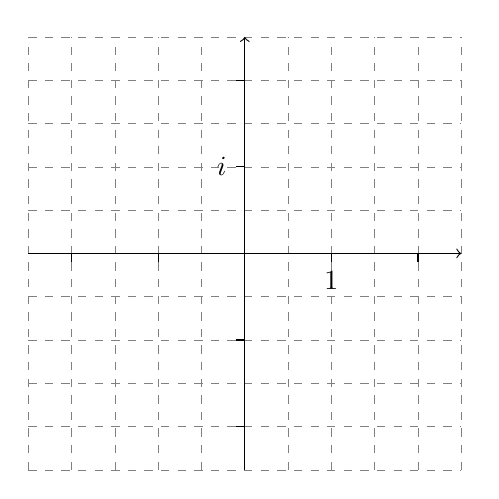
\begin{tikzpicture}[scale = 0.55, even odd rule]
                    % Gitter
                    \draw[dashed, very thin, gray] (-5,-5) grid (5,5);
                    
                    % Achsen mit Skala
                    \draw[->] (-5,0) -- (5,0) node[above] {$\RE$};
                    \draw[->] (0,-5) -- (0,5) node[right] {$\IM$};
                    \foreach \x in {-4,-2,2,4} 
                        \draw (\x,0) -- (\x,-0.2) ;
                     \foreach \y in {-4,-2,2,4}
                        \draw (0,\y) -- (-0.2,\y) ;
                    \draw (0,2) -- (-0.2,2) node[left] {$i$};
                    \draw (2,0) -- (2,-0.2) node[below] {$1$};
                    
                    % % Punkte und Markierungen
                    % \fill[purple!30, opacity=0.5] (0,0) -- (-3,0) arc (180:270:3) -- cycle;
                    % \draw[thick, purple] (0,0) -- (-3,0);
                    % \draw[thick, purple] (0,0) -- (0,-3);
                    

                    % \fill[even odd rule, purple!30, opacity=0.5] (-5,-5) rectangle (5,5) (0,-1) circle (2);
                    % \draw[thick, purple] (0,-1) circle (2);

                \end{tikzpicture}
            \end{center}

\subsubsection*{Juliamengen von Funktionen der Art $f(z) = z^2+c$}
Juliamengen können äussert vielfältig werden. %Bei den folgenden Grafiken ist $D$ dunkel, $E$ hell und $J$ die Randmenge dazwischen.

\begin{figure}[h!]
    \centering
    \begin{subfigure}[t]{0.45\textwidth}
        \centering
        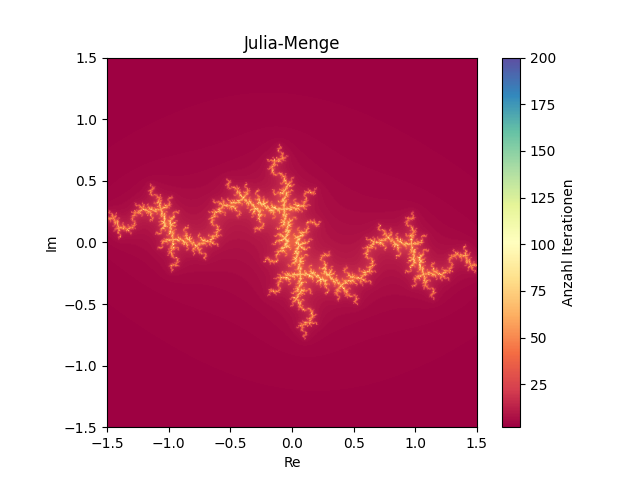
\includegraphics[width=\textwidth]{media/Julia1-spectral.png}
        \caption{Juliamenge für $c=-1+0.3i$}
    \end{subfigure}
    \hfill
    \begin{subfigure}[t]{0.45\textwidth}
        \centering
        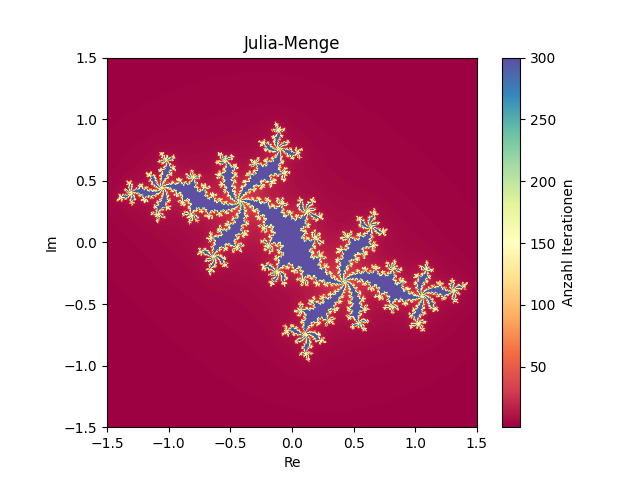
\includegraphics[width=\textwidth]{media/julia2-spectral.png}
        \caption{Juliamenge für $c=-0.5+0.6i$}
    \end{subfigure}
     \begin{subfigure}[t]{0.45\textwidth}
        \centering
        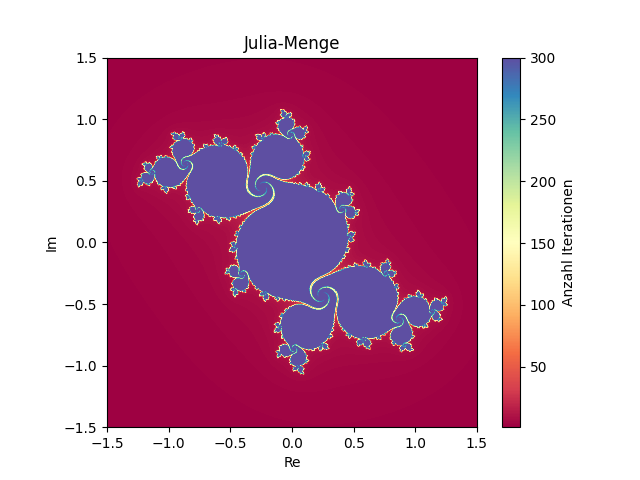
\includegraphics[width=\textwidth]{media/Julia3-spectral.png}
        \caption{Juliamenge für $c=-0.11+0.6557i$}
    \end{subfigure}
    \hfill
    \begin{subfigure}[t]{0.45\textwidth}
        \centering
        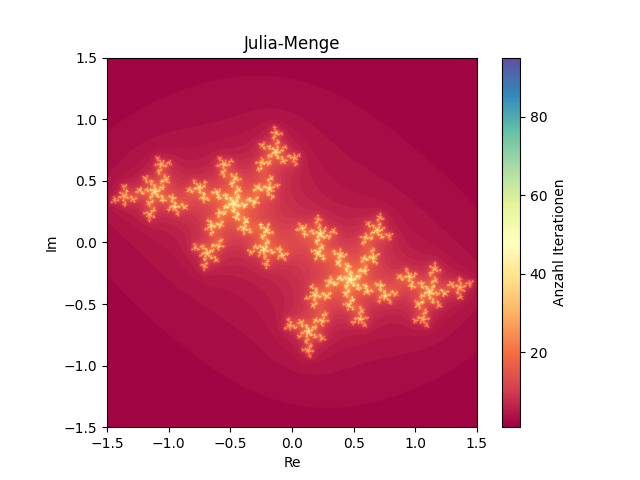
\includegraphics[width=\textwidth]{media/Julia4-spectral.png}
        \caption{Juliamenge für $c=-0.6+0.6i$}
    \end{subfigure}
\end{figure}



\clearpage

Die Bilder oben wurden mit Python erstellt. Das Vorgehen ist grob wie folgt:
\begin{enumerate}
    \item Es wird ein Wert für $c$ in $f(z) = z^2 + c$ festgelegt.
    \item Über einen Bereich der komplexen Zahlenebene (in den Beispielen oben ist es $\RE(z), \IM(z) \in [-1.5, 1.5]$) wird ein feines Gitter gelegt. Jeder Gitterpunkt entspricht dann einem Pixel des Bildes.
    \item Für jeden Gitterpunkt wird die Iteration der Funktion $f$ berechnet. Dabei wird die Anzahl Iterationen bestimmt, die nötig sind, damit der Betrag grösser als eine festgelegte Grenze wird (z. Bsp. 5).
    \item Je nach Anzahl Iterationen wird dem entsprechenden Pixel eine bestimmte Farbe zugeordnet. Damit entsteht eine sogenannte \emph{Heatmap}. Je heller ein Pixel, desto höher ist die Anzahl Iterationen, die nötig waren, damit der Betrag grösser als die Grenze wurde. Je dunkler ein Pixel, desto weniger Iterationen waren nötig.
\end{enumerate}

\begin{LA}
{Heatmaps in Python}{}
Als Erstes müssen Sie sich mit der Bibliothek matplotlib.pyplot vertraut machen. Mit dieser Bibliothek lassen sich Bilder in Python erzeugen.
\begin{enumerate}
    \item Kopieren Sie den folgenden Code und führen Sie ihn aus.
    \lstinputlisting[language=Python]{KomplexeZahlenPython/JuliaMandelbrot/testHeatmap.py}
    \item Verändern Sie das Programm so, dass das Bild eine Art Kreuz darstellt.
\end{enumerate}

Im Folgenden werden Sie einige Optionen des Befehls \lstinline|plt.imshow(bild)| untersuchen.
\begin{enumerate} [resume]
    \item Verändern Sie den Befehl in Zeile 11 wie folgt: \lstinline|plt.imshow(bild,extent=(0, 10, -20, 20))| und beobachten Sie, was passiert.
    \item Der erste Wert \lstinline|bild[0][0]| in der Liste \lstinline|bild| mit dem Wert 1 erscheint in der Grafik ganz oben links. In der Mathematik wird jedoch der Ursprung in der unteren linken Ecke dargestellt. Fügen Sie dem Befehl in Zeile 11 die Option \lstinline|origin='lower'| hinzu, so dass der Befehl wie folgt aussieht: \lstinline|plt.imshow(bild,extent=(0, 10, -20, 20), origin='lower')|. Was passiert nun?
    \item Für die Heatmap gibt es verschiedene Farbskalen. Eine davon ist \lstinline|Spectral|. Fügen Sie dem Befehl in Zeile 11 die Option \lstinline|cmap='Spectral'| hinzu, so dass der Befehl wie folgt aussieht: \lstinline|plt.imshow(bild,extent=(0, 10, -20, 20), origin='lower', cmap='spectral')|. Was passiert nun?
    \item Testen Sie verschiedene Farbskalen. Sie finden Sie in der Dokumentation von \href{https://matplotlib.org/stable/users/explain/colors/colormaps.html}{matplotlib}.
\end{enumerate}

\end{LA}

\begin{LA}
{Programm zur Darstellung der Julia-Menge}{Julia-Menge}
\begin{enumerate}
    \item 
Kopieren Sie das folgende Programm und führen Sie es aus.
\lstinputlisting[language=Python]{KomplexeZahlenPython/JuliaMandelbrot/juliaMenge-V2.py}
\item Diskutieren Sie mit dem*der Banknachbar*in was in den Zeilen 37-46 passiert und beantworten Sie die folgende Frage: Wird das Bild Zeile für Zeile oder Spalte für Spalte aufgebaut?
\item Verändern Sie das Programm so, dass die Julia-Menge für $c = -0.4 + 0.6i$ dargestellt wird.
\item Verändern Sie das Programm so, dass die Julia-Menge der Iteration der Funktion $f(z) = z^3 + c$ berechnet wird.
\end{enumerate}
\end{LA}

\subsubsection*{Mandelbrotmenge}


\begin{definition}
    {Mandelbrotmenge}{}
    Die Mandelbrotmenge ist die Menge aller komplexen Zahlen $c$, für die die Iteration der Funktion $f(z) = z^2 + c$ mit dem Startwert $z_1 = 0$ nicht divergiert.

    Sie wird benannt nach Benoît B. Mandelbrot (1924 - 2010), der sie 1980 entdeckte.
\end{definition}

Mit anderen Worten: Während zur Bestimmung von Juliamengen bei der Funktion $f(z) = z^2 + c$ die Konstante $c$ festgelegt wird und dann die Iteration mit verschiedenen Startwerten $z_1$ untersucht wird, wird bei der Mandelbrotmenge immer mit dem Startwert $z_1 = 0$ gestartet und es werden verschiedene Werte des Parameters $c$ verwendet.

\begin{center}
    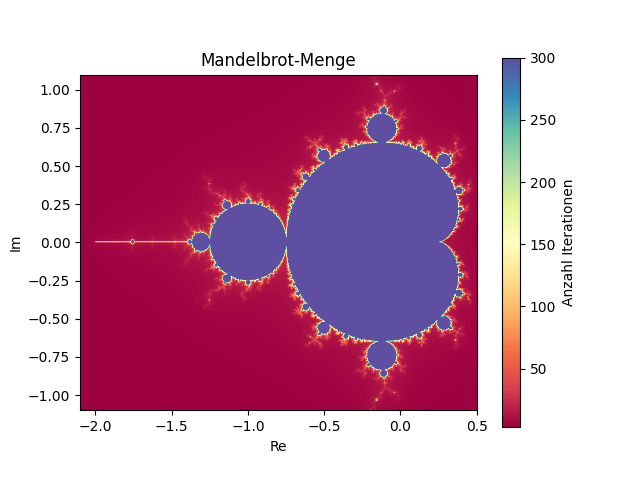
\includegraphics[width = 0.8\textwidth]{media/mandelbrot-spectral.png}
\end{center}

\textbf{Eigenschaften der Mandelbrotmenge $M$:}
\begin{itemize}
    \item $M$ ist ein Fraktal, d. h. es gibt beliebig kleine Ausschnitte von M, welche bei genügender Vergrösserung wieder die Menge M ergeben.
    \item $M$ ist zusammenhängend.
    \item $M$ besteht aus unendlich vielen gleichartigen, selbstähnlichen Teilen. Ein solcher Teil besteht aus einer Herzkurve (Kardioide), an der unendlich viele Kreise angehängt sind. Ferner gehören linienartige Antennen und Fäden zu $M$, welche diese Teile verbinden. Während das Innere der Herzkurve und der Kreise völlig ausgefüllt ist, besteht der Rand aus unbegrenzt vielen, äusserst reichhaltigen Formen.

\end{itemize}
\begin{center}
    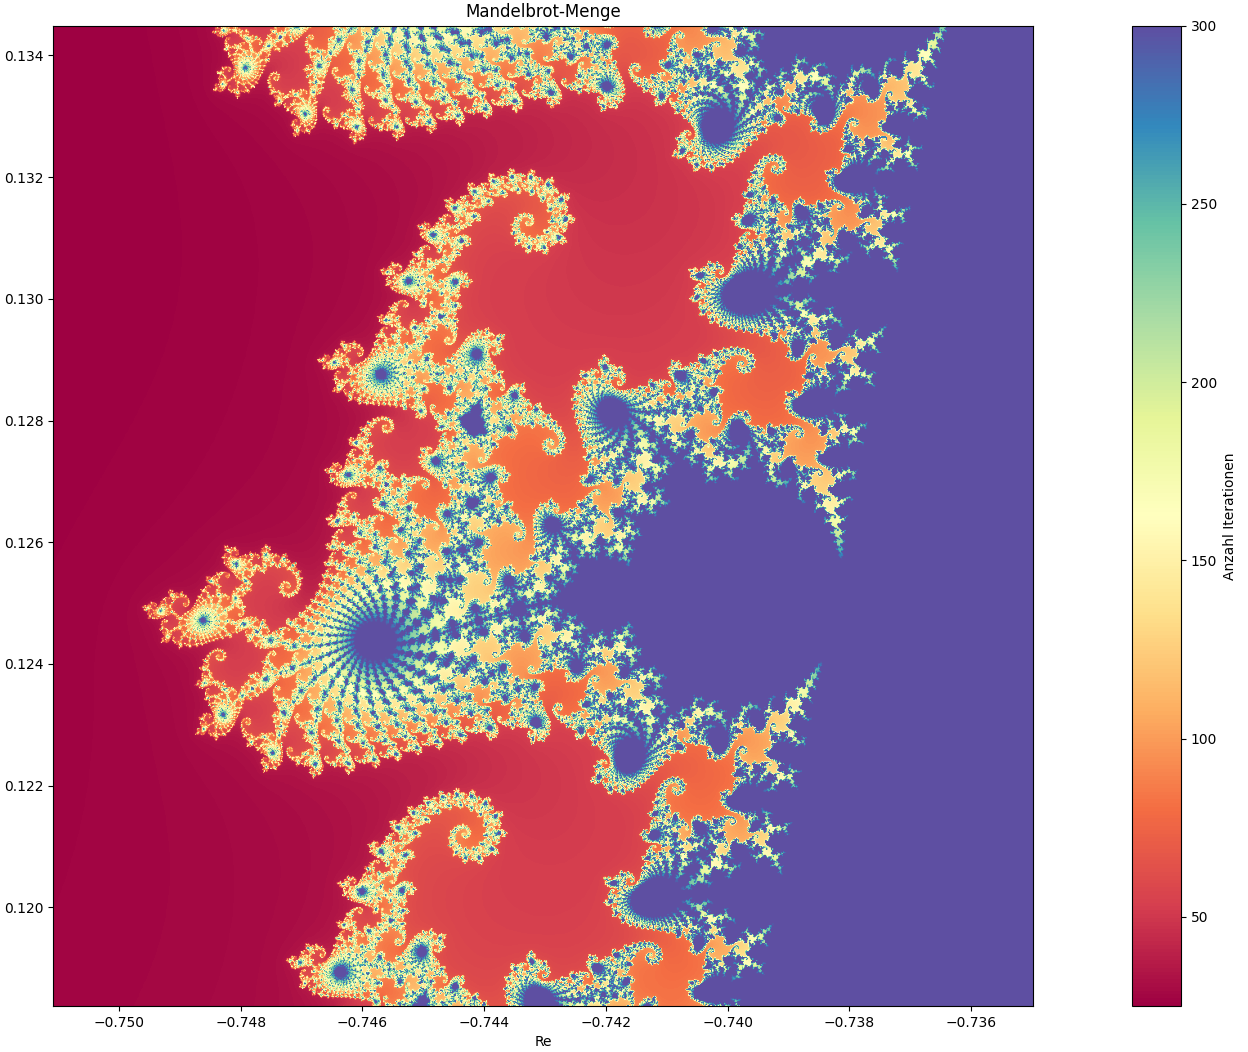
\includegraphics[width = 0.8\textwidth]{media/mandelbrot-zoom3.png}
\end{center}
\begin{ueb}
{Mandelbrotmenge}{}
\begin{enumerate}
    \item Passen Sie das Programm aus der vorherigen \Cref{LA:Julia-Menge} so an, dass die Mandelbrotmenge dargestellt wird. %Verwenden Sie dazu die Funktion $f(z) = z^2 + c$ mit dem Startwert $z_1 = 0$ und variieren Sie den Wert von $c$.
    \item Zoomen Sie in die Mandelbrotmenge hinein, indem Sie den Bereich der komplexen Zahlenebene, der dargestellt wird, verkleinern. Versuchen Sie z.B. den Bereich $\RE(c) = -0.743 566 9 \pm 0.00115$ und $\IM(c) =  0.131 402 3 \pm 0.00115$ darzustellen.

    Je nach Rechenleistung Ihres Computers können Sie die Auflösung des Bildes verändern.
    \item Suchen Sie im Internet nach Video mit den Stichwörtern \emph{Mandelbrot} und \emph{Zoom} und staunen Sie.
\end{enumerate}

\end{ueb}